\section{Census}
\label{sec:census}

OMol-Descriptors-4M comprises $\sim$4 million structures across 34 chemical
verticals, indexing $\sim$1.3M unique compositions. At the
descriptor level the combined corpus carries $\sim$218M atom-level records,
over 30 million charge-scheme records (per-job, per-method), $\sim$1.83 
billion bond-scheme records. All counts in this section are corpus-level
totals prior to the train/val/test partition. Figure~\ref{fig:bond_scheme_breakdown} 
shows the per-vertical bond record
count, decomposed by scheme. Four bond-order schemes are reported on every
structure: Mayer (ORCA), L\"owdin (ORCA), QTAIM, and fuzzy bond order (Multiwfn).
Charge-scheme records track how many partial-charge methods executed
successfully on each structure. The corpus carries $\sim$30M datapoints. 
The full per-vertical breakdown is given in Table~\ref{tab:t1_census}.
Cross-method charge correlations vary substantially by element class:
Hirshfeld--CM5 agreement is the strongest corpus-wide ($R^2 = 0.77$),
while Mulliken and L\"{o}wdin diverge most from the stockholder-partitioned schemes;
pairwise $R^2$ and MAE matrices at the corpus, element-class, and per-vertical levels
are in Appendix~\ref{app:charge_correlations}.


\begin{figure}[h]
\centering
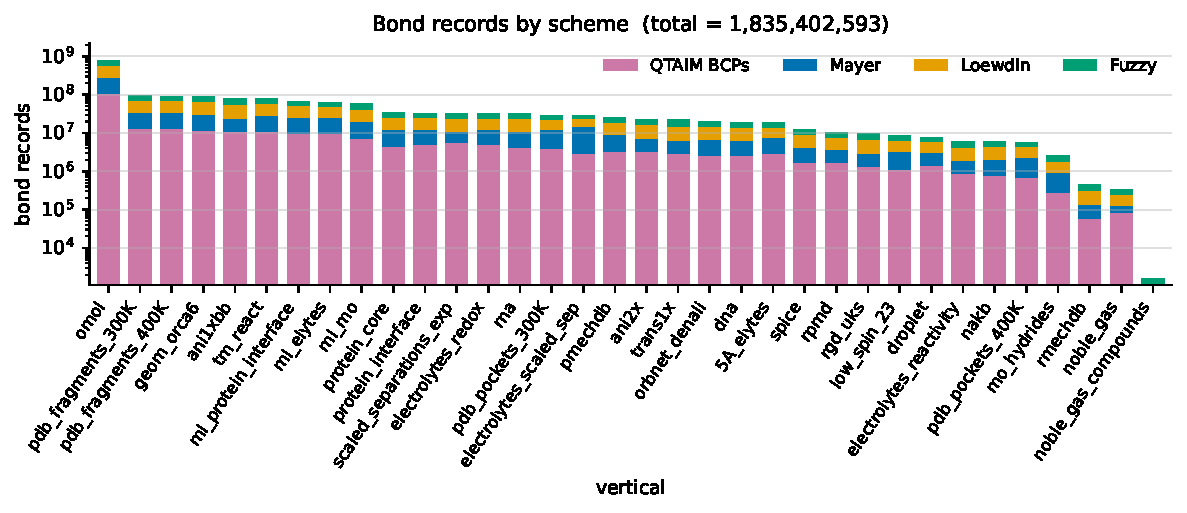
\includegraphics[width=\textwidth]{figures/census/bond_scheme_breakdown.pdf}
\caption{Per-vertical bond-order record counts, stacked by scheme
(QTAIM, Mayer, L\"owdin, fuzzy) on a log axis. Verticals are sorted by total
bond-record count. The four schemes report on the same set of bonds, so
counts represent records, not unique bond instances. Corpus total across
the four schemes is 1.83~billion records.}
\label{fig:bond_scheme_breakdown}
\end{figure}










 

 